
\documentclass[11pt]{article}
\usepackage[margin=1in]{geometry}
\usepackage{graphicx}
\usepackage{booktabs}
\usepackage{float}
\usepackage{hyperref}

\title{Customer Retention Engine}
\author{
Nadir Askarov \and
Valiyyaddin Aliyev \and
Javidan Muradzada \and
Matin Khalilov
}
\date{\today}

\begin{document}
\maketitle
\tableofcontents
\newpage

\section{Problem Overview}
This report summarizes the experiment in \texttt{notebooks/experiment.ipynb}, where the goal is to predict customer churn (\texttt{Churn} = 0/1). The business problem solved by this project is retention management system. Identifying customers likely to churn early and recommending interventions to reduce churn, protect recurring revenue, and prioritize retention operations \texttt{notebooks/recommend.ipynb}. Different classification models were trained and compared, then the best model was selected using F1 score.

\section{Data Description and Cleaning}
The dataset was loaded from:
\begin{center}
\texttt{../data/customer\_churn\_dataset-training-master.csv}
\end{center}

\subsection*{Data sample}
\begin{figure}[H]
\centering
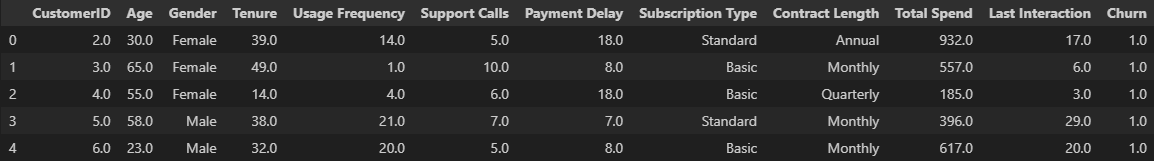
\includegraphics[width=\textwidth]{../figures/data_sample.png}
\caption{Sample rows from the customer churn dataset}
\end{figure}

Initial columns (12):
\texttt{CustomerID, Age, Gender, Tenure, Usage Frequency, Support Calls, Payment Delay, Subscription Type, Contract Length, Total Spend, Last Interaction, Churn}.

\subsection*{Column descriptions}
\begin{table}[H]
\centering
\begin{tabular}{p{3.2cm} p{11.2cm}}
\toprule
\textbf{Column} & \textbf{Description} \\
\midrule
\texttt{CustomerID} & Unique identifier for each customer record. Used only for identification. \\
\texttt{Age} & Customer age in years. Used for exploration and transformed into \texttt{AgeGroup} for modeling. \\
\texttt{Gender} & Customer gender category (e.g., Male/Female). Categorical input feature. \\
\texttt{Tenure} & Duration of customer relationship with the service. Higher/lower values may indicate loyalty differences. \\
\texttt{Usage Frequency} & How frequently the customer uses the service/product. Behavioral engagement signal. \\
\texttt{Support Calls} & Number of customer support interactions. Higher values can indicate dissatisfaction or service issues. \\
\texttt{Payment Delay} & Delay in customer payments. Higher delay can indicate financial or engagement risk. \\
\texttt{Subscription Type} & Plan type selected by the customer (e.g., Basic, Standard, Premium). \\
\texttt{Contract Length} & Billing/contract cycle category (e.g., Monthly, Quarterly, Annual). \\
\texttt{Total Spend} & Total spending amount by customer. \\
\texttt{Last Interaction} & Latest interaction activity . \\
\texttt{Churn} & Target label: 1 = churned customer, 0 = retained customer. \\
\bottomrule
\end{tabular}
\caption{Definitions of all columns in the dataset}
\end{table}

Data quality checks found one row with missing values across all columns. After dropping missing rows:
\[
\texttt{df.shape} = (440832,\ 12)
\]

Then \texttt{CustomerID} was removed because it is an identifier and not a predictive behavioral feature.

\section{Exploratory Data Analysis}
\subsection*{Category distributions}
Key distributions from notebook outputs:
\begin{itemize}
    \item \textbf{AgeGroup}: Senior 156,893; Adult 117,210; Youth 102,693; Child 64,036
    \item \textbf{Gender}: Male 250,252; Female 190,580
    \item \textbf{Subscription Type}: Standard 149,128; Premium 148,678; Basic 143,026
    \item \textbf{Contract Length}: Annual 177,198; Quarterly 176,530; Monthly 87,104
\end{itemize}

\subsection*{Churn-wise averages}
\begin{table}[H]
\centering
\begin{tabular}{lcc}
\toprule
\textbf{Feature} & \textbf{Not Churn (0)} & \textbf{Churn (1)} \\
\midrule
Tenure & 32.2818 & 30.4736 \\
Usage Frequency & 16.2606 & 15.4617 \\
Age & 36.2630 & 41.7473 \\
Payment Delay & 10.0155 & 15.2177 \\
Total Spend & 749.9531 & 541.2855 \\
Support Calls & 1.5864 & 5.1449 \\
\bottomrule
\end{tabular}
\caption{Average feature values by churn class}
\end{table}

Main pattern: churned customers are older on average, have higher payment delay, much more support calls, lower total spend, and slightly lower tenure/usage.

\subsection*{EDA figures}
\begin{figure}[H]
\centering
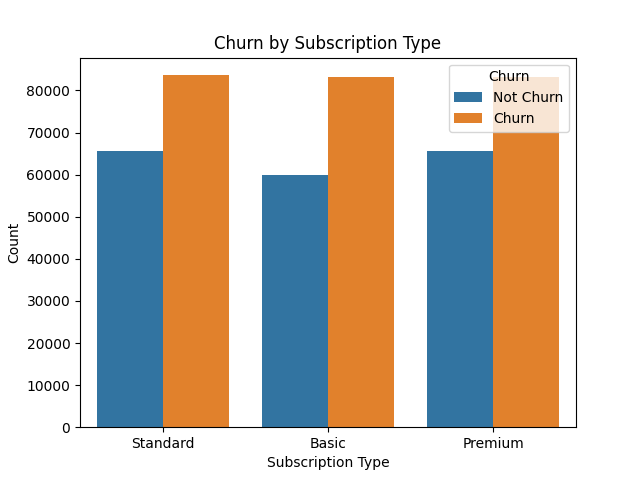
\includegraphics[width=0.75\textwidth]{../figures/churn_by_subscription_type.png}
\caption{Churn counts by subscription type}
\end{figure}

\begin{figure}[H]
\centering
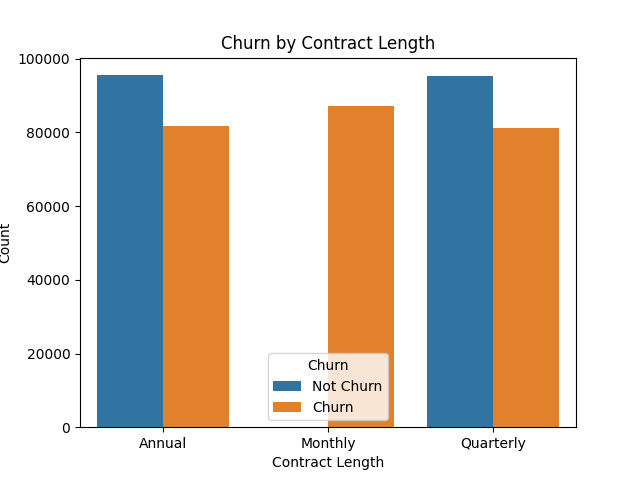
\includegraphics[width=0.75\textwidth]{../figures/churn_by_contract_length.png}
\caption{Churn counts by contract length}
\end{figure}

\section{Feature Engineering and Preprocessing}
\textbf{Implemented feature engineering:}
\begin{itemize}
    \item Created \texttt{AgeGroup} from \texttt{Age} using bins \([15,25), [25,35), [35,45), [45,66)\) with labels \texttt{Child, Youth, Adult, Senior}.
    \item Dropped raw \texttt{Age} from model input after deriving \texttt{AgeGroup}.
\end{itemize}

Model input/target:
\begin{itemize}
    \item \(X = df.drop(['Churn','Age'])\)
    \item \(y = df['Churn'].astype(int)\)
\end{itemize}

Preprocessing pipeline:
\begin{itemize}
    \item \texttt{StandardScaler} for numerical features
    \item \texttt{OneHotEncoder(handle\_unknown='ignore')} for categorical features:
    \texttt{Gender, Subscription Type, Contract Length, AgeGroup}
\end{itemize}

Train/test split:
\begin{itemize}
    \item 80/20 split with \texttt{random\_state=42}, \texttt{stratify=y}
    \item Test support from reports: 88,167 rows (38,167 non-churn, 50,000 churn)
\end{itemize}

\section{Model Building}
To ensure a fair comparison, all models were trained on the same stratified 80/20 split and evaluated on the same test set after identical preprocessing (numerical scaling + categorical one-hot encoding). This design isolates model behavior as the main source of performance differences.

The notebook trained and evaluated four models:
\begin{enumerate}
    \item Logistic Regression (\texttt{max\_iter=1000})
    \item Decision Tree (\texttt{random\_state=42})
    \item Random Forest (\texttt{n\_estimators=100, random\_state=42})
    \item Gradient Boosting (\texttt{n\_estimators=100, random\_state=42})
\end{enumerate}

Each model contributes a different learning bias:
\begin{itemize}
    \item \textbf{Logistic Regression}: linear baseline; useful to check whether churn can be separated with a simple linear boundary.
    \item \textbf{Decision Tree}: captures non-linear thresholds and feature interactions, but can be unstable as a single-tree learner.
    \item \textbf{Random Forest}: bagging ensemble of trees; reduces variance and usually improves generalization on tabular data.
    \item \textbf{Gradient Boosting}: sequentially improves weak learners by focusing on residual errors; often strong on structured datasets.
\end{itemize}

Metrics used for comparison:
\[
\mathrm{Accuracy} = \frac{TP + TN}{TP + TN + FP + FN}, \quad
F1 = \frac{2 \cdot P \cdot R}{P + R}
\]
where \(P\) is precision and \(R\) is recall.

The primary selection criterion is \textbf{F1 score}, because churn prediction requires balancing missed churners (false negatives) and unnecessary interventions (false positives), not only maximizing overall accuracy.

\section{Results and Model Comparison}
\begin{table}[H]
\centering
\begin{tabular}{lcc}
\toprule
\textbf{Model} & \textbf{Accuracy} & \textbf{F1 Score} \\
\midrule
Random Forest & 0.979221 & 0.981407 \\
Gradient Boosting & 0.977509 & 0.979871 \\
Decision Tree & 0.964080 & 0.968420 \\
Logistic Regression & 0.897660 & 0.907845 \\
\bottomrule
\end{tabular}
\caption{Performance comparison from notebook output}
\end{table}

Ranking by F1 is: \textbf{Random Forest} \(>\) \textbf{Gradient Boosting} \(>\) \textbf{Decision Tree} \(>\) \textbf{Logistic Regression}.

Detailed comparison:
\begin{itemize}
    \item \textbf{Random Forest} achieved the best overall performance (Accuracy 0.9792, F1 0.9814).
    \item \textbf{Gradient Boosting} was very close (F1 0.9799), only about 0.0015 below Random Forest.
    \item \textbf{Decision Tree} performed clearly lower than both ensembles (F1 0.9684), showing weaker generalization than ensemble methods.
    \item \textbf{Logistic Regression} had the lowest scores (F1 0.9078), indicating that a linear decision boundary is insufficient for this churn pattern.
\end{itemize}

Class-wise reports and confusion matrices show that ensemble models (Random Forest, Gradient Boosting) reduce both false positives and false negatives compared to single-tree and linear baselines.

\begin{figure}[H]
\centering
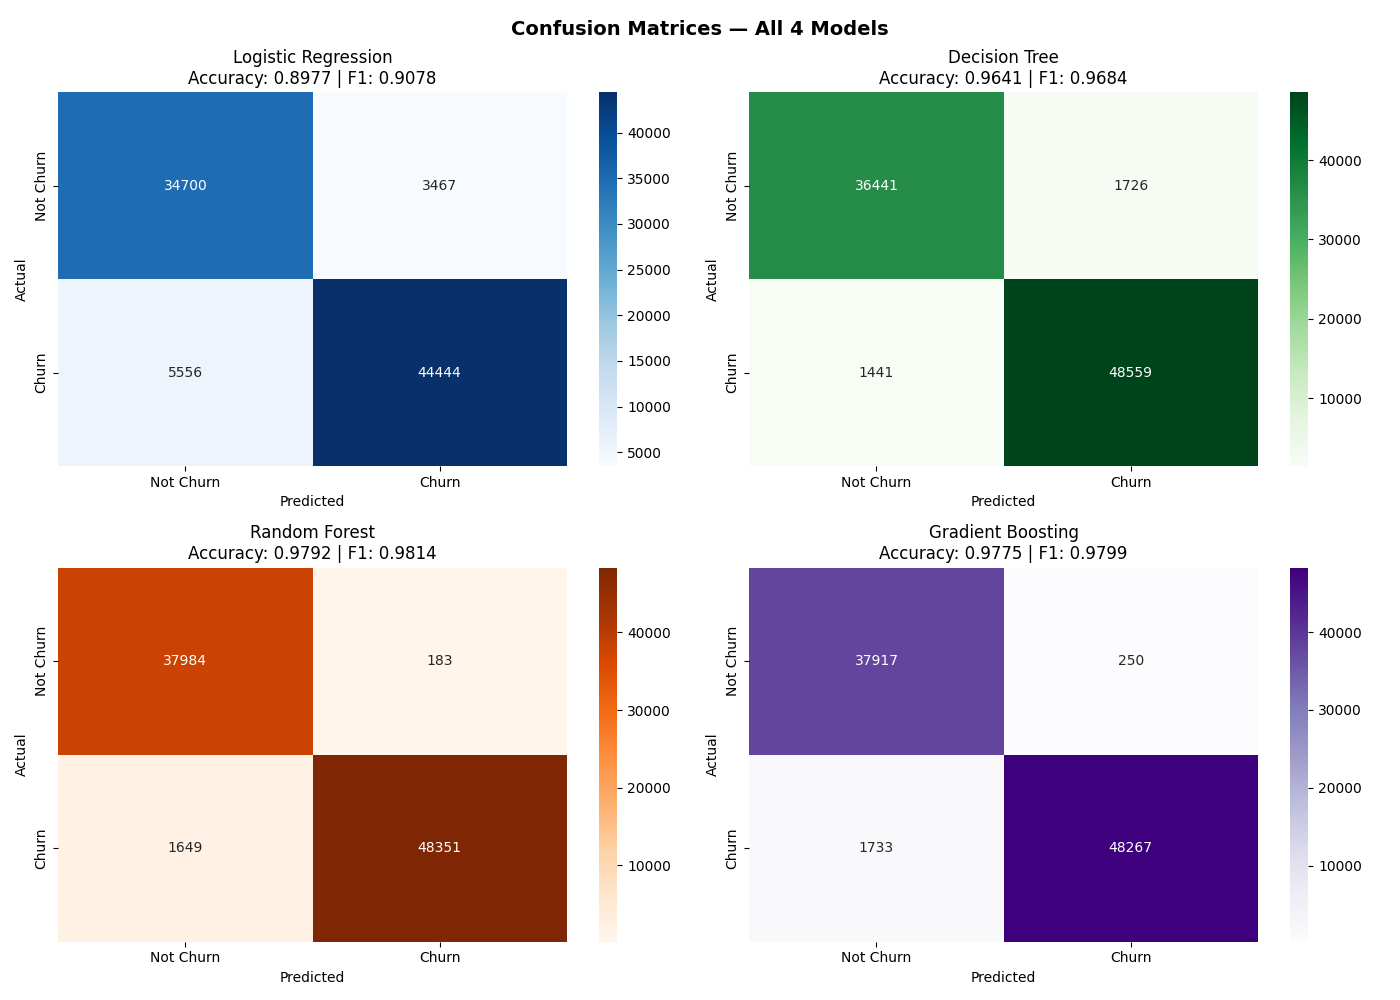
\includegraphics[width=\textwidth]{../figures/confusion_matrices.png}
\caption{Confusion matrices for all four models}
\end{figure}

\section{Best Model Selection}
The final model choice followed a metric-first policy:
\begin{enumerate}
    \item Maximize \textbf{F1 score} (primary business metric for churn intervention quality).
    \item Use \textbf{Accuracy} as a secondary consistency check.
    \item Confirm balanced class-wise behavior from the classification reports and confusion matrix.
\end{enumerate}

Based on this policy, the notebook selected \textbf{Random Forest}:
\begin{itemize}
    \item Accuracy: 0.9792
    \item F1 Score: 0.9814
\end{itemize}

Although Gradient Boosting is highly competitive, Random Forest remains the top model on both reported metrics and therefore becomes the production candidate. The saved artifact (\texttt{best\_model.joblib}) is then used by the recommendation engine to generate customer-level retention actions.

\section{Model Interpretation}
Permutation importance was computed for the selected model.

\begin{figure}[H]
\centering
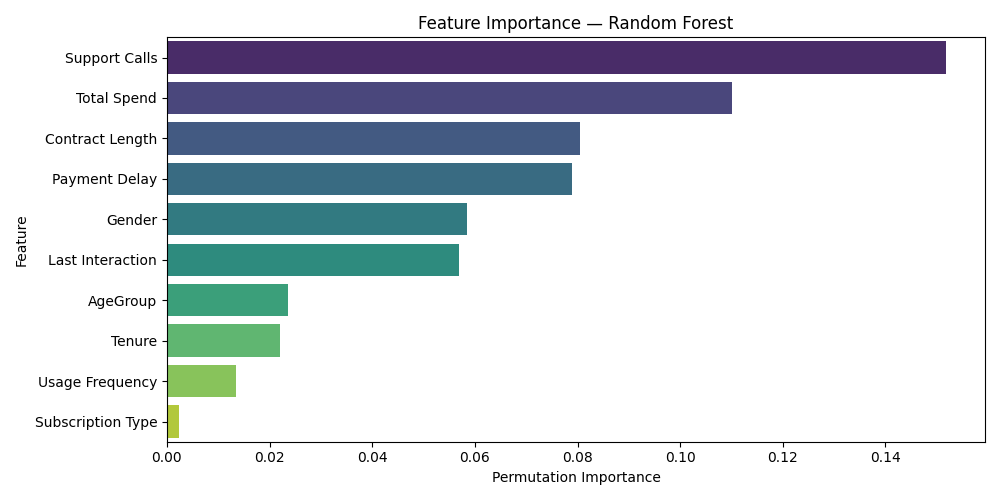
\includegraphics[width=0.9\textwidth]{../figures/feature_importance.png}
\caption{Permutation feature importance for Random Forest}
\end{figure}

Top drivers were:
\begin{enumerate}
    \item Support Calls (0.1518)
    \item Total Spend (0.1102)
    \item Contract Length (0.0804)
    \item Payment Delay (0.0789)
\end{enumerate}

The notebook saved trained artifacts in \texttt{../models/}, including:
\texttt{best\_model.joblib} (Random Forest), all individual models, preprocessing pipeline, and column metadata.

A custom inference example in the notebook used the best model and returned:
\begin{itemize}
    \item Predicted Churn: 0 (Not Churn)
    \item Churn Probability: 0.00\%
    \item Retention Probability: 100.00\%
\end{itemize}

\section{Recommendation System}
After model training, the project adds a \textbf{churn-prevention recommendation engine}. Instead of recommending products, this module recommends \textbf{minimal actionable customer-level interventions} that can flip a predicted outcome from \texttt{Churn} to \texttt{Not Churn}.

\subsection*{Purpose}
For each customer profile:
\begin{enumerate}
    \item Predict churn class and churn probability using the saved best model (Random Forest).
    \item If customer is low risk (\texttt{Not Churn}), return no action.
    \item If customer is high risk (\texttt{Churn}), search for the smallest feasible feature changes that reverse the prediction.
\end{enumerate}

\subsection*{Loaded artifacts and inputs}
The notebook loads:
\begin{itemize}
    \item \texttt{../models/best\_model.joblib}
    \item \texttt{../models/preprocessing\_pipeline.joblib}
    \item \texttt{../models/column\_info.joblib}
\end{itemize}

Model input columns used by this module:
\texttt{Gender, Tenure, Usage Frequency, Support Calls, Payment Delay, Subscription Type, Contract Length, Total Spend, Last Interaction, AgeGroup}.

\subsection*{Actionable retention levers}
\begin{table}[H]
\centering
\begin{tabular}{p{3.8cm} p{2.2cm} p{2.8cm} p{6.0cm}}
\toprule
\textbf{Feature} & \textbf{Direction} & \textbf{Step} & \textbf{Business interpretation} \\
\midrule
\texttt{Total Spend} & Increase & +50 & Offer discount/promo or bundled value to raise spend commitment \\
\texttt{Payment Delay} & Decrease & -1 day & Payment reminders, auto-pay enrollment, billing assistance \\
\texttt{Support Calls} & Decrease & -1 call & Proactive issue resolution to reduce escalations \\
\texttt{Contract Length} & Change category & Monthly/Quarterly/Annual & Move to a more stable contract option when beneficial \\
\bottomrule
\end{tabular}
\caption{Actionable features and intervention logic in \texttt{recommend.ipynb}}
\end{table}

\subsection*{Algorithm design}
The recommendation logic is a \textbf{counterfactual search with greedy minimal changes}:
\begin{enumerate}
    \item Compute baseline prediction and churn probability.
    \item Try each actionable feature independently.
    \item For numeric features, use binary search to find the smallest change that flips prediction.
    \item For contract type, test alternative categories (upgrade path first, then downgrade).
    \item If one feature can flip prediction, pick the lowest-effort single change.
    \item If not, test combinations of 2, 3, ... features and minimize each changed feature while keeping the flipped outcome.
    \item If no feasible intervention flips prediction, return high-risk escalation.
\end{enumerate}

\subsection*{Returned recommendation states}
The engine returns one of four statuses:
\begin{itemize}
    \item \texttt{NO\_ACTION}: customer already predicted as non-churn.
    \item \texttt{SINGLE\_CHANGE}: one minimal intervention is enough.
    \item \texttt{MULTI\_CHANGE}: multiple coordinated interventions are needed.
    \item \texttt{HIGH\_RISK}: model cannot be flipped with allowed actions; escalate to retention team.
\end{itemize}

\subsection*{Worked example from notebook output}
Input customer profile in the notebook:
\begin{center}
\texttt{Female, Tenure=27, Usage Frequency=6, Support Calls=15, Payment Delay=29,}\\
\texttt{Subscription Type=Premium, Contract Length=Quarterly, Total Spend=233,}\\
\texttt{Last Interaction=14, AgeGroup=Adult}
\end{center}

Observed output:
\begin{itemize}
    \item Initial prediction: \textbf{Churn} with probability \textbf{100.00\%}
    \item Recommended status: \texttt{MULTI\_CHANGE}
    \item Coordinated interventions:
    \begin{itemize}
        \item \textbf{Total Spend}: \texttt{233} $\rightarrow$ \texttt{533} \\
        \textit{Business action: Offer discount/promo or bundled value to increase customer commitment and perceived value.}

        \item \textbf{Payment Delay}: \texttt{29} $\rightarrow$ \texttt{20} \\
        \textit{Business action: Apply payment reminders, enable auto-pay, or provide billing assistance to reduce delays.}

        \item \textbf{Support Calls}: \texttt{15} $\rightarrow$ \texttt{4} \\
        \textit{Business action: Proactively resolve issues and improve service quality to reduce repeated support interactions.}
    \end{itemize}
    \item New churn probability after intervention: \textbf{16.00\%}
\end{itemize}

This demonstrates the practical objective of the module: convert model predictions into concrete retention actions with minimal operational effort.

\section{Conclusion}
The pipeline is complete from cleaning and EDA through feature engineering, model comparison, and interpretation. Random Forest achieved the best F1 score and is the final selected model for churn prediction in this project. And recommendation system is used to prevent customer from leaving company

\section*{References}
\begin{enumerate}
    \item L. Breiman, ``Random Forests,'' \textit{Machine Learning}, 45(1), 5--32, 2001.
    \item F. Pedregosa et al., ``Scikit-learn: Machine Learning in Python,'' \textit{Journal of Machine Learning Research}, 12, 2825--2830, 2011. \url{https://scikit-learn.org}
    \item M. Shahid Azeem, ``Customer Churn Dataset,'' Kaggle. \url{https://www.kaggle.com/datasets/muhammadshahidazeem/customer-churn-dataset}
\end{enumerate}

\end{document}
